
\section{Lattice gauge theory and the transfer matrix}\label{sec:lattice}

Write $e_0,\dots,e_3$ for the unit vectors of $\Z^4$, $(x,\mu)$ for the link
from $x$ to $x+e_\mu$, and $Q_{(x,\mu)}^{-1}$ for the variable of the reversed
link. A box $\Lambda$ is a product of four finite intervals, with its set
$E(\Lambda)$ of links and its set $P(\Lambda)$ of plaquettes. For a plaquette
at $x$ in the plane $\mu<\nu$ with links $e_1=(x,\mu)$, $e_2=(x+e_\mu,\nu)$,
$e_3=(x+e_\nu,\mu)$, $e_4=(x,\nu)$, put $Q_p=Q_{e_1}Q_{e_2}Q_{e_3}^*Q_{e_4}^*$.
With $dQ$ the Haar probability measure of $G$, the Wilson measure of a box
with free boundary is
\[
W_\Lambda(dQ)=\frac1{Z_\Lambda}\exp\Bigl(N\beta\sum_{p\in P(\Lambda)}\ReTr
Q_p\Bigr)\prod_{e\in E(\Lambda)}dQ_e ,
\]
and the Wilson measure $\mu_L$ of the torus $\Lambda_L=(\Z/L\Z)^4$ is defined
in the same way with all links and plaquettes of $\Lambda_L$. Both are
invariant under the gauge transformations $Q_{(x,y)}\mapsto g_xQ_{(x,y)}
g_y^{-1}$. A function of finitely many links is a local observable, and it
is gauge invariant if it is invariant under these transformations. For
$\beta\ge0$ the measures are reflection positive for reflections in lattice
hyperplanes through sites and in hyperplanes bisecting links, on boxes
symmetric under the reflection and on tori of even side~\cite{OSei78}.

Let $\omega$ be a state on the gauge-invariant local observables of $\Z^4$
that is invariant under translations and reflection positive in this sense.
The Osterwalder--Schrader construction~\cite{OS73,OS75,OSei78} gives a
Hilbert space $\mathcal H$ with a unit vector $\Omega$, a map $F\mapsto\Psi_F$
from the observables at nonnegative times to $\mathcal H$ with dense range,
and a self-adjoint transfer matrix $0\le\mathbb T\le1$ with $\mathbb T\Omega=
\Omega$ and
\[
\ip{\Psi_F}{\mathbb T^t\Psi_H}=\omega\bigl(\vartheta(\bar F)\,\tau_tH\bigr),
\qquad t\in\Z_{\ge0},
\]
where $\vartheta$ is the time reflection and $\tau_t$ the time translation;
$\Psi_F$ is the class of $F$ for the positive semidefinite form
$\omega(\vartheta(\bar F)H)$, and $\|\Psi_F\|^2\le\omega(|F|^2)$. The
\emph{spectral gap} of $\mathbb T$ is $m$ if its spectrum on $\Omega^\perp$
lies in $[0,e^{-m}]$.

\begin{proposition}\label{prop:gapdecay}
Let $m>0$ and let $\mathcal F$ be a class of gauge-invariant local
observables, supported at nonnegative times, that is dense in $L^2(\omega)$
on each bounded time support. If for every $F\in\mathcal F$ there is
$C_F<\infty$ with
\[
\omega(\vartheta(\bar F)\tau_tF)-|\omega(F)|^2\le C_Fe^{-mt}\qquad(t\ge0),
\]
then $\mathbb T$ has spectral gap at least $m$.
\end{proposition}

\begin{proof}
Put $\Psi'_F=\Psi_F-\ip\Omega{\Psi_F}\Omega$, so that the left side equals
$\ip{\Psi'_F}{\mathbb T^t\Psi'_F}=\int\lambda^t\,d\sigma_F(\lambda)$, with
$\sigma_F$ the spectral measure of $\mathbb T$ at $\Psi'_F$. For $\delta>0$
this is at least $\sigma_F((e^{-m+\delta},1])e^{(-m+\delta)t}$, which exceeds
$C_Fe^{-mt}$ for large $t$ unless $\sigma_F((e^{-m+\delta},1])=0$. So the
spectral projection of $(e^{-m},1]$ annihilates every $\Psi'_F$. These vectors
are dense in $\Omega^\perp$, because $\|\Psi_F\|^2\le\omega(|F|^2)$ and the
class is dense, so the projection vanishes on $\Omega^\perp$.
\end{proof}

The decay of a single two-point function does not suffice: it places only
one spectral measure in $[0,e^{-m}]$, and the density of the class is what
gives the gap.

\section{The line field}\label{sec:linefield}

A \emph{direction field} is a map $\sigma:\Z^4\to\{0,1,2,3\}$; its links
are $F=\{(x,\sigma(x)):x\in\Z^4\}$. At each site put $\pi_x(\mu)=
\sigma(x+e_\mu)$. The plaquette at $x$ in the plane $\{\mu,\nu\}$ contains
\begin{equation}\label{eq:count}
[\sigma(x)\in\{\mu,\nu\}]+[\pi_x(\mu)=\nu]+[\pi_x(\nu)=\mu]
\end{equation}
links of $F$.

\begin{lemma}\label{lem:cycle}
Every plaquette contains exactly one link of $F$ if and only if, at every
site $x$, $\pi_x$ fixes $\sigma(x)$ and permutes the other three directions
cyclically.
\end{lemma}

\begin{proof}
Fix $x$, let $s=\sigma(x)$ and let $R$ be the other three directions. For the
plane $\{s,\nu\}$ the count~\eqref{eq:count} is $1+[\pi_x(s)=\nu]+[\pi_x(\nu)
=s]$, which equals one for all $\nu\in R$ exactly when $\pi_x$ fixes $s$ and
maps $R$ into $R$. For a plane $\{\mu,\nu\}\subset R$ the count is
$[\pi_x(\mu)=\nu]+[\pi_x(\nu)=\mu]$. Draw an arrow $\mu\to\pi_x(\mu)$ whenever
$\pi_x(\mu)\in R\setminus\{\mu\}$; each vertex has at most one outgoing arrow,
and the condition asks for exactly one arrow on each of the three pairs. Three
arrows on three vertices with out-degree at most one give out-degree one
everywhere, and such a tournament is a directed three-cycle.
\end{proof}

From now on $\sigma$ is the field of period two of Table~\ref{tab:sigma} in
Appendix~\ref{app:table}; in each row $\pi_x$ fixes $\sigma(x)$ and is a
three-cycle on the other directions, so every plaquette contains exactly one
link of $F$.\footnote{A field with one link of $F$ at every site and one in
every plaquette can exist only in four dimensions: a site carries
$d(d-1)/2$ plaquettes at which it is the base point and a link lies in
$2(d-1)$ plaquettes, and the two counts agree only for $d=4$.} Call the links
outside $F$ \emph{active} and write $A$ for their set.

\begin{lemma}\label{lem:structure}\leavevmode
\begin{enumerate}[label=\textup{(\roman*)},leftmargin=*]
\item $F$ is a disjoint union of bi-infinite straight lines, one through every
site; hence $F\cap E(\Lambda)$ is a forest for every box $\Lambda$.
\item An active link $e=(x,\mu)$ lies in six plaquettes. In four of them the
link of $F$ shares an end point with $e$; in the other two it is opposite to
$e$.
\item Every active link shares a plaquette with exactly twelve other active
links, two in each of its plaquettes, and two links share at most one
plaquette.
\end{enumerate}
\end{lemma}

\begin{proof}
(i) Since $\pi_x$ fixes $\sigma(x)$, $\sigma(x+e_{\sigma(x)})=\sigma(x)$, and since
$\sigma$ has period two, also $\sigma(x-e_{\sigma(x)})=\sigma(x)$. If $(x-e_\nu,\nu)
\in F$, straightness at $x-e_\nu$ gives $\sigma(x)=\nu$, so the incoming link of
$F$ at $x$ is unique and continues the outgoing one. A line meets a box in a
segment.

(ii) A link of $F$ sharing an end point with $e$ is the outgoing or incoming
link of $F$ at $x$, of direction $s=\sigma(x)\ne\mu$, or at $x+e_\mu$, of
direction $t=\pi_x(\mu)\in R\setminus\{\mu\}$. They lie in the two plaquettes of
$e$ in the plane $\{\mu,s\}$ and the two in the plane $\{\mu,t\}$, four distinct
plaquettes as $s\ne t$. In the two plaquettes of the remaining plane
$\{\mu,\rho\}$ the unique link of $F$ touches neither end of $e$, so it is the
opposite link.

(iii) Each plaquette of $e$ contains $e$, one link of $F$ and two other links.
\end{proof}

\begin{figure}[t]
\centering
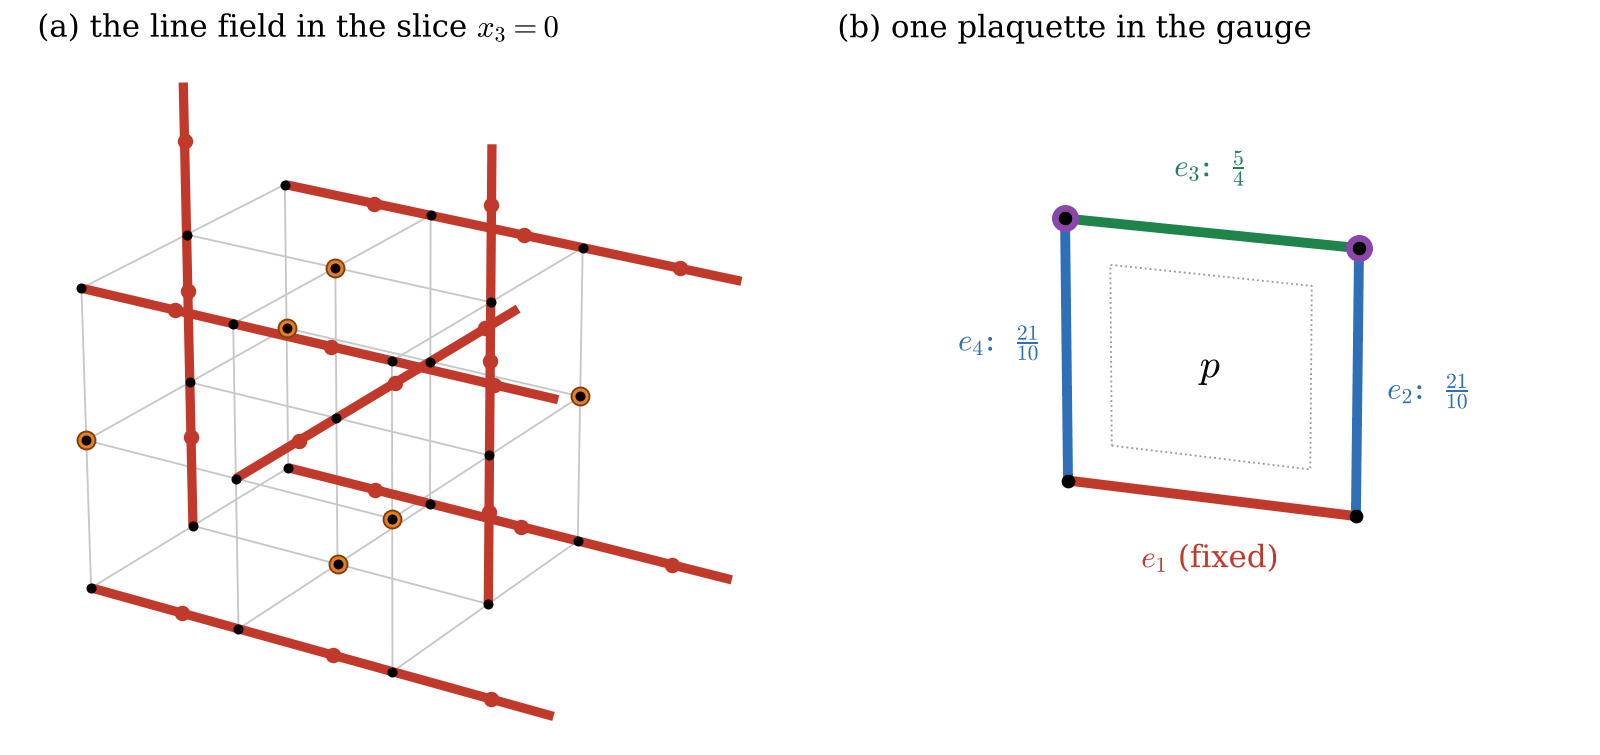
\includegraphics[width=0.92\textwidth]{fig_linefield.png}
\caption{(a) The line field in the slice $x_3=0$ of a box of side three;
thick segments are links of $F$, rings mark sites whose line leaves the slice
in direction $3$. (b) One plaquette with its fixed link $e_1$ and the weights
$\frac{21}{10}$, $\frac54$ of Lemma~\ref{lem:local} on its active links.}
\label{fig:linefield}
\end{figure}

\section{Gauge fixing and the free-boundary state}\label{sec:state}

For a function $O$ of the links let $O^F$ be $O$ with every link of $F$ set to
the identity.

\begin{lemma}[gauge fixing]\label{lem:gaugefix}
Let $\mu^F_\Lambda$ be the probability measure on $G^{A\cap E(\Lambda)}$ with
density proportional to $\exp(N\beta\sum_{p\in P(\Lambda)}\ReTr Q^F_p)$. For
every gauge-invariant $O$ on $G^{E(\Lambda)}$, $W_\Lambda(O)=\mu^F_\Lambda(O^F)$.
\end{lemma}

\begin{proof}
Each segment of $F\cap E(\Lambda)$ is a path $x_0,\dots,x_k$. Given the
variables on $F$, put $g_{x_0}=1$ and $g_{x_{i+1}}=g_{x_i}Q_{(x_i,x_{i+1})}$
along every segment. The transformed field equals the identity on $F\cap
E(\Lambda)$, and for fixed values on $F$ the map from the active variables to
the transformed ones is a product of translations, which preserve Haar
measure. Gauge invariance of the action and of $O$ gives the claim.
\end{proof}

No holonomy remains because $F\cap E(\Lambda)$ is a forest. The measures
$\mu^F_\Lambda$ are finite-volume versions of the specification $\gamma^F$ on
$G^A$ in which $\gamma^F_e$ resamples an active $Q_e$ from the law with density
proportional to $\exp(N\beta\sum_{p\ni e}\ReTr Q^F_p)$ given the other active
links. Fix a bi-invariant metric $\delta$ on $G$ of diameter $D$ and define the
Kantorovich coefficients
\[
C_{ee'}=\sup\frac{W_1\bigl(\gamma^F_e(\cdot\mid Q),\gamma^F_e(\cdot\mid Q')\bigr)}
{\delta(Q_{e'},Q'_{e'})},
\]
the supremum over configurations that differ only at $e'$; $W_1$ is the
Kantorovich distance~\cite{Vil09}, and $C_{ee'}=0$ unless $e$ and $e'$ share a
plaquette.

\begin{lemma}[comparison]\label{lem:comparison}
Suppose every row and column of $(C_{ee'})$ sums to at most $\alpha<1$, and let
$\lambda>0$ with $\theta=\alpha e^\lambda<1$. Let $S\subset A$ and let $\mu_1,\mu_2$
be probability measures on $G^A$ invariant under $\gamma^F_e$ for $e\notin S$.
Let $T\subset A\setminus S$ be finite, $w_b=e^{-\lambda\dist(b,T)}$ with the
distance of link midpoints, and suppose $\sum_{z\in S}w_z<\infty$. There is a
coupling of $\mu_1$ and $\mu_2$ with $\varrho(b)=\E\,\delta(\sigma_b,\sigma'_b)$
satisfying
\[
\sum_{b\notin S}w_b\varrho(b)\le\frac{\theta D}{1-\theta}\sum_{z\in S}w_z ,
\]
and $\mu_1=\mu_2$ if $S=\emptyset$.
\end{lemma}

\begin{proof}
The couplings form a weakly compact set on which $\Psi(\pi)=\sum_bw_b\E_\pi
\delta(\sigma_b,\sigma'_b)$ is continuous; let $\pi^*$ minimise it. For $e\notin S$
replace $(\sigma_e,\sigma'_e)$ by a sample of an optimal coupling of
$\gamma^F_e(\cdot\mid\sigma)$ and $\gamma^F_e(\cdot\mid\sigma')$, chosen
measurably~\cite[Cor.~5.22]{Vil09}. Both $\mu_i$ are invariant, so this is again
a coupling, and changing the links that enter $\gamma^F_e$ one at a time gives
$\varrho(e)\le\sum_{e'}C_{ee'}\varrho(e')$ by minimality. Multiply by $w_e$ and sum
over $e\notin S$; where $C_{ee'}\ne0$, $w_e\le e^\lambda w_{e'}$, so
$\sum_{e\notin S}w_e\varrho(e)\le\theta[\sum_{e'\notin S}w_{e'}\varrho(e')+D\sum_{z
\in S}w_z]$. If $S=\emptyset$ this forces $\varrho\equiv0$.
\end{proof}

Conditioning on the links of the support of $H$~\cite[Ch.~3]{Kal21} and
applying the lemma to the two conditional measures gives, for the Gibbs
measure $\mu$ of $\gamma^F$, a local $F'$ that is $L$-Lipschitz in each link and
a bounded $H$ with finite support disjoint from that of $F'$,
\begin{equation}\label{eq:decay}
|\Cov_\mu(F',H)|\le\|H\|_\infty L\,\frac{\theta D}{1-\theta}\,|\operatorname{supp}H|\,
e^{-\lambda\dist(\operatorname{supp}F',\operatorname{supp}H)} .
\end{equation}

\begin{proposition}\label{prop:state}
Suppose every row and column of $(C_{ee'})$ sums to at most $\alpha<1$. Then
$\gamma^F$ has a unique Gibbs measure $\mu_F$; for every gauge-invariant local $O$
the limit $\omega(O)=\lim W_\Lambda(O)$ exists along every sequence of boxes
exhausting $\Z^4$ and equals $\mu_F(O^F)$; $\omega$ is invariant under
translations and the hypercubic group; truncated correlations of Lipschitz
gauge-invariant observables decay at every rate below $-\log\alpha$; and for
$\beta\ge0$, $\omega$ is reflection positive and its transfer matrix has
spectral gap at least $-\log\alpha$.
\end{proposition}

\begin{proof}
Gibbs measures exist by compactness and coincide by Lemma~\ref{lem:comparison}
with $S=\emptyset$. Extend $\mu^F_\Lambda$ by Haar measure outside $\Lambda$ and
let $S$ be the set of active links with a plaquette outside $P(\Lambda)$; off $S$
the extended measure is invariant under $\gamma^F_e$. Lemma~\ref{lem:comparison}
with $T$ the support of $O^F$ bounds $|\mu^F_\Lambda(O^F)-\mu_F(O^F)|$ by
$C_TR^3e^{-\lambda R}$, $R$ the distance from $T$ to the complement of $\Lambda$,
for Lipschitz $O$, and uniform approximation handles continuous $O$;
Lemma~\ref{lem:gaugefix} identifies $\mu^F_\Lambda(O^F)$ with $W_\Lambda(O)$. Since
$W_\Lambda(\tau_vO)=W_{\Lambda-v}(O)$ and the limit does not depend on the
exhausting sequence, $\omega$ is invariant; the line field is a device for
computing $W_\Lambda$ and is never moved. Reflection positivity of $W_\Lambda$ on
symmetric boxes passes to the limit. The decay is~\eqref{eq:decay}, since
$\Cov_\omega(O,O')=\Cov_{\mu_F}(O^F,O'^F)$. Lipschitz gauge-invariant functions
are dense in the gauge-invariant part of $L^2(\omega)$ on every support, being
Lipschitz functions on the compact quotient by the gauge group, so
Proposition~\ref{prop:gapdecay} gives the gap.
\end{proof}

\begin{proof}[Proof of Theorem~\ref{thm:A} for $\SU(2)$]
Identify $\SU(2)$ with the unit quaternions and use the chordal metric. For an
active link $e$ and a plaquette $p\ni e$ let $s_p$ be the product of the other
three variables, ordered so that $\operatorname{Re}(Q_es_p)=\frac12\Tr Q_p$, with
links of $F$ equal to one. Since $N\beta\ReTr Q_p=4\beta\ip{Q_e}{\bar s_p}$ in
$\R^4$, the conditional law of $Q_e$ is the von Mises--Fisher law $\nu_b(dx)
\propto e^{\ip xb}dx$ on $S^3$ with $b=4\beta\sum_{p\ni e}\bar s_p$. Moving a
partner $e'$ by $\delta$ moves one staple by an isometric image of that
displacement, hence $b$ by $4|\beta|\delta$, and the sharp
quarter of~\cite{BB26a}, $W_1(\nu_b,\nu_{b'})\le\frac14|b-b'|$, gives
$C_{ee'}\le|\beta|$. By Lemma~\ref{lem:structure}(iii) every row and column has
twelve nonzero entries, so $\alpha\le12|\beta|=3|\beta_W|$, and
Proposition~\ref{prop:state} applies for $|\beta_W|<\frac13$.
\end{proof}

The value $\frac13$ is the end of this argument: at $b=0$ the derivative of
$\nu_b$ has Kantorovich norm exactly $\frac14$, the six staples of an active
link can be arranged with sum zero while one of them moves freely, and so
every row sum of the matrix is exactly $3|\beta_W|$. Without the gauge every
link has eighteen partners and the same argument stops at $\beta_W=\frac29$
\cite[Prop.~13]{BB26a}.
